
%%%%%%%%%%%%%%%%%%%%%%%%%%%%%%%%%%%%%%%%%%%%%%%%%%%%%%%%%%%%%%%%%%%%%%%%%%%%%%%%%%%%%%%%%%%%%%%%%%%%%%%%%%%%%%%%%%%%%%%%%%
% Project Report/Thesis LaTeX Template
% Christ University - M.Tech Project Report
%%%%%%%%%%%%%%%%%%%%%%%%%%%%%%%%%%%%%%%%%%%%%%%%%%%%%%%%%%%%%%%%%%%%%%%%%%%%%%%%%%%%%%%%%%%%%%%%%%%%%%%%%%%%%%%%%%%%%%%%%%

%----------------------------------------------------------------------------------------
%	PACKAGES AND OTHER DOCUMENT CONFIGURATIONS
%----------------------------------------------------------------------------------------

\documentclass[12pt, oneside]{Thesis} % The default font size and one-sided printing

\graphicspath{{Pictures/}} % Specifies the directory where pictures are stored

\usepackage[square, numbers, comma, sort&compress]{natbib}
\hypersetup{urlcolor=blue, colorlinks=true}
\title{\ttitle}

\usepackage{mathptmx, imakeidx, hyperref, listings, color, textcomp, algorithm, pdfpages, setspace, imakeidx, datetime, ragged2e}
\usepackage[numbers]{natbib}
\usepackage{amsmath,amssymb}

\makeindex

\hypersetup{%
	colorlinks=true,
	linkcolor=black}

\usepackage[noend]{algpseudocode}
\algrenewcommand\Return{\State \algorithmicreturn{} }

\definecolor{listinggray}{gray}{0.9}
\definecolor{lbcolor}{rgb}{0.9,0.9,0.9}
\lstset{
	backgroundcolor=\color{lbcolor},
	tabsize=4,
	rulecolor=,
	language=python,
	basicstyle=\scriptsize,
	upquote=true,
	aboveskip={1.5\baselineskip},
	columns=fixed,
	showstringspaces=false,
	extendedchars=true,
	breaklines=true,
	prebreak = \raisebox{0ex}[0ex][0ex]{\ensuremath{\hookleftarrow}},
	frame=single,
	showtabs=false,
	showspaces=false,
	showstringspaces=false,
	identifierstyle=\ttfamily,
	keywordstyle=\color[rgb]{0,0,1},
	commentstyle=\color[rgb]{0.133,0.545,0.133},
	stringstyle=\color[rgb]{0.627,0.126,0.941},
}

\makeindex[intoc]

\begin{document}
	

% All the Variable should be entered inside {}

% Name of the University
\newcommand{\UniversityName}
{CHRIST (Deemed to be University)}

% Name of the department only
\newcommand{\DepartmentName}
{Department of AI and Data Science Engineering}

% Title of the project or thesis
\newcommand{\ProjectTitle}
{Regime-Aware Multi-Asset Volatility Forecasting using Temporal Fusion Transformers}

% Type of Dissertation M.Tech Dissertation or B.Tech Dissertation
\newcommand{\DissertationType}
{A Project Report on}

% Program name: MASTER OF TECHNOLOGY or BACHELOR OF TECHNOLOGY in Uppercase
\newcommand{\ProgramNameUpper}
{MASTER OF TECHNOLOGY}

% Program name: Master of Technology or Bachelor of Technology in Normal case
\newcommand{\ProgramName}
{Master of Technology}

% Program Short form: M.Tech. or B.Tech.
\newcommand{\ProgramNameShort}
{M.Tech.}

% Specialization
\newcommand{\SpecializationName}
{AI and Data Science Engineering}

% Name of Student
\newcommand{\AuthorNameOne}
{Abhishek Deep}

\newcommand{\RegisterNoOne}
{2462023}

% Name of the Guide
\newcommand{\GuideName}
{Dr. Alpha Vijayan}

% Designation of the Guide
\newcommand{\GuideDesignation}
{Assistant Professor}

% Department of Guide where he belongs to
\newcommand{\GuideDepartment}
{\DepartmentName}

% Name of the Co-Guide
\newcommand{\CoGuideName}
{}

% Designation of the Co-Guide
\newcommand{\CoGuideDesignation}
{}

% Department of Co-Guide where he belongs to
\newcommand{\CoGuideDepartment}
{\DepartmentName}

\newcommand{\NameofAuthortobeCertified}
{Abhishek Deep}

% Leave blank in {} if co-guide is not there
\newcommand{\CoGuideAnd}
{}

% Address of the department
\newcommand{\DepartmentNameAddress}
{
\textbf{\large{
	\DepartmentName\\ 
	School of Engineering and Technology \\ \UniversityName\\ 
	Kumbalgodu,\,Bangalore\,-\,560~074
}}
} 

% Project Date
\newcommand{\ProjectDate}
{March-2026}

% Academic Year
\newcommand{\AcademicYear}
{2025-2026}

% Name of the College
\newcommand{\CollegeName}
{School of Engineering and Technology}

% Name of the HOD or Coordinator
\newcommand{\HODorCoordinator}
{Dr. Balamurugan M}

% Name of the Position of the Head
\newcommand{\HODorCoordinatorDesignation}
{Head of Department}

% Name of the Vice-Chancellor
\newcommand{\VCName}
{Dr. Rev. Fr. Jose C C}

% Name of the Pro Vice Chancellor
\newcommand{\ProVCName}
{Dr. Rev. Fr. Viju P D}

% Name of the Director of the College
\newcommand{\DirectorName}
{Dr. Rev. Fr Sony J. Chundattu}

% Name of the Dean/Associate Dean
\newcommand{\DeanName}
{Dr. E A Mary Anita}

% Name of the Position of Dean/Associate Dean
\newcommand{\DeanDesignation}
{Assoc. Dean}

% 'We' or 'I'
\newcommand{\WeorI}
{I}

% Acknowledgement for Guide
\newcommand{\AcknowledgementForGuide}
{
	\WeorI~am also extremely grateful to my guide, \textbf{\GuideName}, for her constant support, guidance, and encouragement throughout this project. Her expertise in machine learning and data science has been instrumental in shaping this work.\\
}

% Acknowledgement for Co-Guide (Leave blank if no co-guide) 
\newcommand{\AcknowledgementForCoGuide}
{}

% Acknowledgement for Others
\newcommand{\AcknowledgementForOthers}
{
    \WeorI~would also like to express my heartfelt gratitude to my parents for their unwavering support, encouragement, and blessings throughout the course of this project.
}

% Date of Declaration
\newcommand{\DateofDeclaration}
{March 2026}


\frontmatter

\setstretch{1.5}

\fancyhead{}
\rhead{\thepage}
\lhead{}

\pagestyle{fancy}

\newcommand{\HRule}{\rule{\linewidth}{0.5mm}}

% PDF meta-data
\hypersetup{pdftitle={\ProjectTitle}}
\hypersetup{pdfsubject=\SpecializationName}
\hypersetup{pdfauthor=\AuthorNameOne}
\hypersetup{pdfkeywords=\GuideName \\ \DepartmentName}

%----------------------------------------------------------------------------------------
%	TITLE PAGE
%----------------------------------------------------------------------------------------

\begin{titlepage}
	
\begin{center}
		\begin{figure}[!hb]
			\centering {{
\includegraphics[totalheight=1.4in]{Christ.jpg}}}
		\end{figure}
	{\Large{\DissertationType}} \\
	\vspace{0.2in}
	{\Large \textbf{\textrm{\ProjectTitle}}}\\
	\vspace{0.2in}
	{Submitted in partial fulfillment of the requirements
	for the degree of }\\

	{\large{{\textbf{\textrm{ \ProgramNameUpper\\}}}}}

	{\large{{\textbf{\textrm{in\\}}}}}
	
	{\large{{\textbf{\textrm{ \SpecializationName\\}}}}}

	{\large{by}}\\

	\begin{tabular}{cc}
			{\large{\textrm{\textbf{\AuthorNameOne}}}} & {\large{~\RegisterNoOne}}\\
	\end{tabular}

	\vspace{0.1cm}
	

	\vspace{0.5cm}
	{\large{Under the Guidance of}}\\
	\vspace{0.1cm} {\large{\textrm{\textbf{\GuideName}
					\\}}} \vspace{3.0cm}
	
		\DepartmentNameAddress 
	\ProjectDate
\end{center}

\end{titlepage}

\clearpage

\fancyhead[]{}
\renewcommand\footrulewidth{0pt}
\renewcommand\headrulewidth{0pt} 

\fancypagestyle{plain}{
	\fancyhead{}
	\fancyfoot[R]{\thepage}
}

%----------------------------------------------------------------------------------------
%	University Vision
%----------------------------------------------------------------------------------------

% Uvision.tex (safe include)
% Note: no \cleardoublepage here; let the main document control page breaks.

\clearpage
\thispagestyle{empty}

\begingroup
\centering

{\Large\bfseries Vision}\par\vspace{0.75em}
\emph{``Excellence and Service''}\par\vspace{1.5em}

{\Large\bfseries Mission}\par\vspace{0.75em}
\begin{minipage}{0.85\textwidth}
\centering
\emph{``CHRIST (Deemed to be University) is a nurturing ground for an individual's holistic development to make effective contribution to the society in a dynamic environment.''}
\end{minipage}\par\vspace{1.75em}

{\Large\bfseries Core Values}\par\vspace{0.75em}
\begin{minipage}{0.6\textwidth}
\raggedright
\begin{itemize}
\item Faith in God
\item Moral Uprightness
\item Love of Fellow Beings
\item Social Responsibility
\item Pursuit of Excellence
\end{itemize}
\end{minipage}

\endgroup
\clearpage


%----------------------------------------------------------------------------------------
%	Department Vision
%----------------------------------------------------------------------------------------

% Dvision.tex (safe include)
% Note: no \cleardoublepage here; let the main document control page breaks.

\clearpage
\thispagestyle{empty}

\begingroup
\centering

{\Large\bfseries Department Vision}\par\vspace{0.75em}
\emph{``To fortify Ethical Computational Excellence''}\par\vspace{1.5em}

{\Large\bfseries Department Mission}\par\vspace{0.75em}
\begin{minipage}{0.9\textwidth}
\raggedright
\begin{enumerate}
\item[M1:] Imparts core and contemporary knowledge in the areas of Computation and Information Technology.
\item[M2:] Promotes the culture of research and facilitates higher studies.
\item[M3:] Acquaints the students with the latest industrial practices, team building and entrepreneurship.
\item[M4:] Sensitizes the students to serve for environmental, social \& ethical needs of society through lifelong learning.
\end{enumerate}
\end{minipage}\par\vspace{1.5em}

{\Large\bfseries Program Educational Objectives (PEOs)}\par\vspace{0.75em}
\begin{minipage}{0.9\textwidth}
\raggedright
\begin{enumerate}
\item[PEO1:] \textbf{Professional Acumen:} Understand, analyze and design solutions with professional competency for real world problems.
\item[PEO2:] \textbf{Critical Analysis:} Develop software/embedded solutions for the requirements, based on critical analysis and research.
\item[PEO3:] \textbf{Team work:} Function effectively in a team and as an individual in a multidisciplinary/multicultural environment.
\item[PEO4:] \textbf{Life Long Learning:} Accomplish holistic development comprehending professional responsibilities.
\end{enumerate}
\end{minipage}

\endgroup
\clearpage


%----------------------------------------------------------------------------------------
%	Certificate Page
%----------------------------------------------------------------------------------------

\input{Primitives/Certificate}

%----------------------------------------------------------------------------------------
%	Bonafide Certificate Page
%----------------------------------------------------------------------------------------

\newpage
\BonafideCertificate{
\begin{center}
		\begin{figure}[!hb]
			\centering {{
\includegraphics[totalheight=1.4in]{Christ.jpg}}}
		\end{figure}

		\textbf{{\LARGE{{\textrm{ \CollegeName\\}}}}}

		{\Large{{\textrm{ \DepartmentName\\}}}}
			\vspace{0.5in}
		{\Large \textbf{\textrm{BONAFIDE CERTIFICATE}}}\\
\end{center}		
		
		\justify
		{
		It is to certify that this project titled "\ProjectTitle" is the bonafide work of  \\
	}
	
	\begin{center}
		\begin{tabular}{cc}
			\hline
			{\large{\textrm{\textbf{Name}}}} & {\large{~\textbf{Register Number}}}
			\\
			\hline
			{\large{\textrm{\textbf{\AuthorNameOne}}}} & {\large{~\RegisterNoOne}}\\
		\end{tabular}
	\end{center}
	
	
\begin{center}	
	
	\begin{tabular}{p{6cm} p{0.25cm} p{5cm}}
			\vspace{0.5cm} &  \\
		\textbf{Examiners [Name and Signature]}&&  Name of the Candidate :\\
		1.&& Register Number           : \\
		2.&& Date of Examination     : \\

	\end{tabular}


\end{center}

}


%----------------------------------------------------------------------------------------
%	ACKNOWLEDGEMENTS
%----------------------------------------------------------------------------------------

\setstretch{1.3}

\acknowledgements{\addtocontents{toc}{\vspace{1em}}

\WeorI~would like to thank Vice Chancellor \textbf{\VCName }, \UniversityName, Pro Vice Chancellor \textbf{\ProVCName}, Director of \CollegeName \textbf { Dr. Fr. Jiby Jose E}, Assistant Director \textbf{Fr. Shijin P J}, Dean \textbf{Dr. Raghunandan Kumar R} and the Associate Dean \textbf{Dr. Mary Anita E A} for their kind patronage. \\

\WeorI~would like to express my sincere gratitude and appreciation to the \HODorCoordinatorDesignation~of~\DepartmentName,~\CollegeName~ \textbf{\HODorCoordinator}, for giving me this opportunity to take up this project. \\

\AcknowledgementForGuide  \\
\AcknowledgementForOthers \\

}

\clearpage

%----------------------------------------------------------------------------------------
%	DECLARATION PAGE
%----------------------------------------------------------------------------------------

\Declaration{

	
	\WeorI, Hereby declare that the Project titled "\textbf{\ProjectTitle}" is a record of original project work undertaken by me for the award of the degree of \textbf{\ProgramName}~in~\textbf{\SpecializationName}. I have completed this study under the supervision of \textbf{\GuideName}, \GuideDepartment.\\
	
	\WeorI~also declare that this project report has not been submitted for the award of any degree, diploma, associateship, fellowship or other title anywhere else. It has not been sent for any publication or presentation purpose.
	
	\textbf{Place:} \CollegeName, \UniversityName, Bangalore \\
	\textbf{Date:} \DateofDeclaration
	
	\begin{center}
		\begin{tabular}{ccp{5cm}}
			\hline
			{\large{\textrm{\textbf{Name}}}} & {\large{~\textbf{Register Number}}}
			&{\large{~\textbf{~~~~~~~~~~~~Signature}}}\\
			\hline
			&&\\
			{\large{\textrm{\textbf{\AuthorNameOne}}}} & {\large{~\RegisterNoOne}} &\\
			&&\\
		\end{tabular}
	\end{center}
}


\clearpage

%----------------------------------------------------------------------------------------
%	ABSTRACT PAGE
%----------------------------------------------------------------------------------------

\abstract{\addtocontents{toc}{\vspace{1em}} 
	
	Accurately predicting volatility in stock markets is a challenging issue in computational finance, especially in emerging economies where structural breaks and regime switches are commonplace. This project presents a Regime-Aware Temporal Fusion Transformer (RA-TFT) framework designed for next-day realized volatility forecasting across 14 stocks listed on the National Stock Exchange (NSE) of India. Leveraging approximately 2.65 million five-minute OHLCV observations collected over nearly a decade, we integrate Hidden Markov Model (HMM)-derived regime labels, GARCH(1,1) conditional volatility, and DCC-inspired cross-asset correlations into a 47-feature input set processed by the TFT architecture.

	A controlled ablation study separates autoregressive persistence from genuine feature-driven prediction. Model~A (with the autoregressive target input) achieves $R^2 = 0.976$ and MAPE of 1.90\%, closely matching HAR-RV baselines. Model~B (without autoregressive input) yields $R^2 = 0.258$, confirming that engineered features carry modest but genuine predictive information beyond lagged volatility. Regime-conditioned evaluation shows strong performance in low-through-high volatility states ($R^2 > 0.98$), with degradation during extreme events ($R^2 = 0.765$). The TFT's Variable Selection Network reveals that lagged daily realized volatility dominates all other features by two orders of magnitude, effectively rediscovering the HAR-RV structure from data.
	\\ 
	
	\textbf{Keywords:} Volatility Forecasting, Temporal Fusion Transformer, Hidden Markov Model, GARCH, Indian Stock Market, Deep Learning
}

\clearpage


%----------------------------------------------------------------------------------------
%	LIST OF CONTENTS/FIGURES/TABLES PAGES
%----------------------------------------------------------------------------------------

\pagestyle{fancy}

\tableofcontents

\lhead{\emph{List of Figures}}
\listoffigures

\lhead{\emph{List of Tables}}
\listoftables

%----------------------------------------------------------------------------------------
%	THESIS CONTENT - CHAPTERS
%----------------------------------------------------------------------------------------

\mainmatter

\pagestyle{fancy}

\fancyhead[]{}
\renewcommand\footrulewidth{0pt}
\renewcommand\headrulewidth{0pt}
\fancyfoot[R]{\thepage}

\chapter{INTRODUCTION}
\label{ChapterIntroduction}

\section{Background and Motivation}

The ability to anticipate future price movements is central to the way modern finance is conducted. From establishing appropriate risk limits to the valuation of derivative contracts, market participants constantly try to get accurate forecasts of volatility. Volatility, which quantifies the degree to which returns vary in the market, is important for quantifying portfolio risk, establishing option prices through the Black-Scholes framework, and determining capital adequacy ratios under Basel~III regulatory requirements.

Traditional econometric models have long served as the primary tools for volatility estimation and forecasting. The Generalized Autoregressive Conditional Heteroskedasticity (GARCH) family of models \cite{bollerslev1986} captures the well-documented phenomenon of volatility clustering, where periods of high and low volatility tend to persist. However, typical GARCH specifications assume parametric distributions for innovations and are inherently univariate. These limitations mean that cross-asset spillovers and non-linear dynamics often go unmodelled. Corsi's Heterogeneous Autoregressive model of Realized Volatility (HAR-RV) \cite{corsi2009} tackles well the long-memory property of volatility through its multi-horizon lag structure, but the linearity assumption remains a constraint.

Deep learning models like Long Short-Term Memory (LSTM) networks and Transformer-based architectures have shown strong capabilities in time series forecasting. Nevertheless, the practical implementation of these models in quantitative finance has been hindered by a lack of model transparency. Risk managers and regulators who need to understand why a model makes specific predictions often cannot trust a black-box system. Lim et al. \cite{lim2021} proposed the Temporal Fusion Transformer (TFT) as an interpretable alternative that combines Variable Selection Networks with multi-head attention, allowing direct inspection of feature importance and temporal attention patterns.

The Indian stock market presents unique challenges for volatility forecasting. As one of the largest emerging markets globally, the National Stock Exchange (NSE) of India exhibits distinct characteristics including higher volatility clustering, greater susceptibility to global shocks, and periodic regime transitions driven by both domestic policy changes and international capital flows. These features make it an ideal test bed for regime-aware forecasting approaches.

\section{Problem Statement}

Despite advances in deep learning for financial time series, several critical gaps remain in the volatility forecasting literature:

\begin{itemize}
    \item Most existing deep learning approaches for volatility forecasting operate as black-box models, providing little insight into which features drive predictions.
    \item Few studies systematically separate the contribution of autoregressive persistence from genuine feature-driven prediction in deep learning volatility models.
    \item The application of advanced attention-based architectures like the TFT to high-frequency realized volatility forecasting on Indian equity markets remains unexplored.
    \item Market regime information is seldom integrated directly with deep learning volatility models, despite substantial evidence that volatility dynamics differ across market states.
\end{itemize}

This project addresses these gaps by developing a regime-aware forecasting framework that combines the interpretability advantages of the TFT with statistical regime detection and classical volatility features.

\section{Objectives}

The main objectives of this project are:

\begin{enumerate}
    \item To develop a multi-asset learning framework using TFT for joint modeling of 14 NSE equities, incorporating regime-aware conditioning through HMM-derived state labels.
    \item To conduct a controlled ablation study that separates autocorrelation persistence from genuine feature-based prediction in the context of realized volatility forecasting.
    \item To perform detailed interpretability analysis via the TFT's Variable Selection Network, identifying which features and time steps drive volatility predictions.
    \item To evaluate the model's performance across different market regimes (low, normal, high, and extreme volatility) using regime-conditioned metrics.
    \item To benchmark the proposed RA-TFT framework against established classical baselines including HAR-RV and GARCH family models.
\end{enumerate}

\section{Scope of the Project}

The scope of this project encompasses:

\begin{itemize}
    \item \textbf{Data:} Five-minute OHLCV (Open-High-Low-Close-Volume) data for 14 liquid NSE equities spanning approximately 10 years, totaling approximately 2.65 million observations.
    \item \textbf{Feature Engineering:} Construction of 47 features across six categories including multi-scale realized volatility, HAR-RV lags, jump detection statistics, range-based estimators, GARCH and cross-asset features, and temporal encodings.
    \item \textbf{Modeling:} Implementation of the TFT architecture with two ablation variants (Model A with autoregressive input, Model B without), along with HAR-RV and GARCH family baselines.
    \item \textbf{Evaluation:} Comprehensive evaluation using $R^2$, RMSE, MAPE, Directional Accuracy, and QLIKE metrics, with regime-conditioned performance analysis.
\end{itemize}

\section{Organization of the Report}

This report is organized as follows:

\begin{itemize}
    \item \textbf{Chapter 2: Literature Survey} reviews classical volatility models, deep learning approaches for volatility forecasting, and regime-switching methodologies.
    \item \textbf{Chapter 3: Research Methodology} describes the data collection, feature engineering pipeline, model architecture, training configuration, and evaluation framework.
    \item \textbf{Chapter 4: Actual Work} details the implementation of the system architecture, feature extraction modules, model training, and regime detection.
    \item \textbf{Chapter 5: Results, Discussions and Conclusions} presents the experimental results, regime-conditioned analysis, interpretability findings, and conclusions with future work.
\end{itemize}

\chapter{LITERATURE SURVEY}
\label{ChapterLiteratureSurvey}

Volatility forecasting has been a central topic in financial econometrics for over four decades. This chapter surveys the evolution from classical parametric models through deep learning approaches and regime-switching methodologies, providing the foundation for the proposed Regime-Aware Temporal Fusion Transformer framework.

\section{Literature Collection \& Segregation}

The literature for this project was collected from leading academic databases including IEEE Xplore, ScienceDirect, Springer, SSRN, and Google Scholar. The search focused on three primary domains: (1) volatility forecasting models, (2) deep learning for financial time series, and (3) regime-switching approaches. Over 80 papers were initially identified, from which 22 were selected based on relevance, recency, and methodological contribution.

The selected literature was segregated into three categories:
\begin{itemize}
    \item \textbf{Classical Volatility Models:} Foundational econometric approaches including ARCH, GARCH, and realized volatility models.
    \item \textbf{Deep Learning for Volatility:} Neural network architectures applied to volatility prediction, including LSTM, attention-based RNNs, and Transformers.
    \item \textbf{Regime-Switching and Interpretable Architectures:} Hidden Markov Models, regime-aware strategies, and the TFT architecture.
\end{itemize}

\section{Critical Review of Literature}

\subsection{Classical Volatility Models}

The field of volatility modelling began with the seminal work of Engle \cite{engle1982}, who introduced the Autoregressive Conditional Heteroskedasticity (ARCH) model demonstrating that time-varying variance could be modelled as a function of past squared residuals. Bollerslev \cite{bollerslev1986} extended this into the Generalized ARCH (GARCH) framework, which added lagged conditional variance terms and became the most widely used parametric volatility model in practice.

Recognizing that negative returns tend to increase volatility more than positive returns of equal magnitude---the so-called leverage effect---Nelson \cite{nelson1991} proposed the Exponential GARCH (EGARCH) model. This model uses logarithmic conditional variance, allowing asymmetric effects without requiring non-negativity constraints. Similarly, Glosten, Jagannathan, and Runkle \cite{glosten1993} introduced the GJR-GARCH model with an explicit indicator function for negative shocks.

The availability of high-frequency data enabled the development of realized volatility measures as a non-parametric alternative to GARCH. Parkinson \cite{parkinson1980} proposed an efficient estimator using only daily high and low prices, while Garman and Klass \cite{garman1980} incorporated opening and closing prices for improved efficiency. Rogers and Satchell \cite{rogers1991} developed an estimator robust to drift in the underlying process. Barndorff-Nielsen and Shephard \cite{bns2004} introduced bipower variation as a means to separate the continuous and jump components of return variation.

Corsi's Heterogeneous Autoregressive model of Realized Volatility (HAR-RV) \cite{corsi2009} uses daily, weekly, and monthly lagged RV as regressors in a simple linear framework. Despite its simplicity, HAR-RV remains the dominant benchmark in realized volatility forecasting due to its ability to capture long-memory patterns through the heterogeneous lag structure. In our dataset, HAR-RV achieves $R^2 > 0.98$, setting a demanding benchmark.

\subsection{Deep Learning for Volatility Forecasting}

The application of deep learning to financial volatility forecasting has grown rapidly. Bucci \cite{bucci2020} provided an early systematic comparison showing that LSTM networks outperform traditional GARCH models in daily volatility forecasting, particularly during crisis periods. The ability of LSTMs to capture long-range dependencies through their gating mechanism makes them naturally suited for volatility time series.

Kim and Won \cite{kim2022} advanced this line of research by incorporating attention mechanisms into RNN architectures. Their attention-augmented models better focus on informative lookback periods, thereby improving realized-volatility $R^2$. This work demonstrated that not all historical observations are equally relevant for volatility prediction---some time steps carry significantly more predictive information.

Wu et al. \cite{wu2023} experimented with standard encoder-decoder Transformers for multi-step volatility prediction on US stocks, reporting clear improvements over both HAR-RV and LSTM baselines. Their study highlighted the advantages of self-attention for capturing complex temporal dependencies in volatility dynamics.

Hybrid approaches that combine classical econometric intuition with neural network flexibility have shown particular promise. Zhang et al. \cite{zhang2023} proposed a GARCH-informed neural network which embeds the GARCH variance equation into the inductive bias of the deep network, ensuring that the model respects known volatility dynamics while learning additional non-linear patterns. Rahimikia and Poon \cite{rahimikia2023} incorporated news sentiment scores alongside price features into a machine learning pipeline and demonstrated that textual information carries volatility-relevant value beyond what price data alone provides.

Christensen et al. \cite{christensen2023} conducted a comprehensive survey of machine learning approaches to volatility forecasting, concluding that neural networks and gradient-boosted trees consistently outperform linear benchmarks, with the largest gains observed during periods of market stress.

\subsection{Regime-Switching Models and the TFT Architecture}

Hamilton \cite{hamilton1989} pioneered the application of Markov-switching dynamics to economic time series, providing a principled framework for modelling structural breaks. In the volatility forecasting context, regime-switching models allow different parameterizations for calm, normal, and stressed market conditions. Nystrup et al. \cite{nystrup2021} demonstrated that portfolio strategies driven by HMM-identified regimes significantly improve risk-adjusted returns, motivating the direct integration of regime labels into forecasting models.

The Temporal Fusion Transformer, introduced by Lim et al. \cite{lim2021}, represents a significant advance in interpretable time series forecasting. The architecture combines several key components: Variable Selection Networks that learn instance-specific feature weights, Gated Residual Networks for effective non-linear processing, a seq2seq structure with LSTM encoder-decoder, and multi-head interpretable attention. This combination provides both accurate forecasts and transparent explanations.

Olorunnimbe and Viktor \cite{olorunnimbe2023} applied the TFT to equity price prediction, demonstrating that the variable-selection outputs provide portfolio managers with actionable insights about which factors are driving market dynamics. Chen et al. \cite{chen2024} extended TFT applications to cryptocurrency markets, showing that the architecture transfers well despite the very different microstructure of digital asset markets.

Patel and Sharma \cite{patel2024} examined volatility forecasting in emerging markets using a hybrid regime-aware deep learning framework, while Zhao et al. \cite{zhao2024} proposed an attention-based multi-scale volatility predictor that works directly with high-frequency data, demonstrating the benefits of multi-resolution feature extraction.

\subsection{Summary of Literature Review}

Table \ref{tab:litreview} summarizes the key contributions reviewed in this chapter.

\begin{table}[h!]
\caption{Summary of Key Literature Reviewed}
\label{tab:litreview}
\centering
\small
\begin{tabular}{p{3.5cm}p{2cm}p{6cm}}
\hline
\textbf{Author(s)} & \textbf{Year} & \textbf{Key Contribution} \\
\hline
Engle & 1982 & Introduced ARCH for time-varying variance \\
Bollerslev & 1986 & Generalized ARCH to GARCH framework \\
Hamilton & 1989 & Markov-switching for economic time series \\
Corsi & 2009 & HAR-RV model for realized volatility \\
Bucci & 2020 & LSTM outperforms GARCH for daily RV \\
Lim et al. & 2021 & Temporal Fusion Transformer architecture \\
Kim \& Won & 2022 & Attention-augmented RNNs for volatility \\
Wu et al. & 2023 & Transformer surpasses HAR-RV and LSTM \\
Zhang et al. & 2023 & GARCH-informed neural networks \\
Christensen et al. & 2023 & ML consistently beats linear benchmarks \\
\hline
\end{tabular}
\end{table}

\section{Research Gap}

While significant progress has been made in both deep learning volatility forecasting and regime-switching models, several gaps remain:

\begin{enumerate}
    \item No existing study has applied the TFT architecture specifically to intraday realized volatility forecasting on Indian equities.
    \item The contribution of autoregressive persistence versus genuine feature-driven prediction in deep learning volatility models has rarely been systematically quantified through controlled ablation.
    \item Direct integration of HMM regime labels as conditioning features within the TFT framework has not been explored.
    \item Cross-stock variation in feature-driven predictability remains poorly understood, particularly in emerging market contexts.
\end{enumerate}

This project addresses these gaps through the proposed Regime-Aware Temporal Fusion Transformer framework.

\chapter{RESEARCH METHODOLOGY}
\label{ChapterResearchMethodology}

This chapter describes the research methodology adopted for the entire project, including data collection, feature engineering, model architecture design, training procedures, and evaluation framework.

\section{Research Design Overview}

The project follows an experimental research design with the following phases:

\begin{enumerate}
    \item \textbf{Data Collection:} Acquisition and preprocessing of high-frequency intraday data from the NSE.
    \item \textbf{Feature Engineering:} Construction of 47 features from raw OHLCV data organized into six categories.
    \item \textbf{Regime Detection:} Application of Hidden Markov Models for market state identification.
    \item \textbf{Model Development:} Implementation of the TFT architecture with two ablation variants.
    \item \textbf{Baseline Benchmarking:} Implementation of HAR-RV and GARCH family baselines.
    \item \textbf{Evaluation:} Comprehensive performance assessment using multiple metrics across regime conditions.
\end{enumerate}

\section{Dataset Description}

The dataset comprises 5-minute Open-High-Low-Close-Volume (OHLCV) data from fourteen highly liquid equities listed on the National Stock Exchange of India. The chosen securities represent multiple sectors to ensure diverse volatility dynamics:

\begin{itemize}
    \item \textbf{Banking:} HDFCBANK, ICICIBANK, AXISBANK, SBIN
    \item \textbf{Information Technology:} INFY, TCS, WIPRO
    \item \textbf{Energy:} RELIANCE, COALINDIA
    \item \textbf{Infrastructure:} LT, ADANIPORTS
    \item \textbf{Defence:} HAL
    \item \textbf{Metals:} TATASTEEL
    \item \textbf{Consumer:} TITAN
\end{itemize}

The dataset spans approximately ten years, giving $\sim$194,000 bars per stock and approximately 2.65 million rows in total. Indian equity trading runs from 9:15~AM to 3:30~PM IST, yielding 75 five-minute bars per trading day.

\subsection{Data Preprocessing}

The raw data underwent several preprocessing steps:

\begin{enumerate}
    \item \textbf{Outlier Removal:} Price bars with returns exceeding 10 standard deviations from the rolling mean were flagged and corrected using linear interpolation.
    \item \textbf{Missing Value Imputation:} Gaps in the time series (due to trading halts, data feed issues) were filled using forward-fill for prices and zero-fill for volumes.
    \item \textbf{Intraday Seasonality Adjustment:} The well-documented U-shaped intraday volatility pattern (high at open, low mid-day, rising toward close) was accounted for through normalization.
    \item \textbf{Train-Validation Split:} A strictly chronological split was enforced with no random shuffling, ensuring temporal integrity.
\end{enumerate}

\section{Feature Engineering Pipeline}

A total of 47 features were engineered from the raw price and volume data, organized into six categories as described below.

\subsection{Multi-Scale Realized Volatility}

Realized volatility is computed as the square root of the sum of squared high-frequency intraday returns $(r_{t,i})$:

\begin{equation}
RV_h = \sqrt{\sum_{i=1}^{h} r_{t,i}^2} \times \sqrt{252}
\end{equation}

This is annualized and calculated over multiple horizons: $h \in \{12, 38, 75, 375\}$ bars, corresponding to approximately 1 hour, half-day, 1 day, and 1 week respectively. This multi-scale approach captures volatility dynamics at different temporal resolutions.

\subsection{HAR-RV Lag Features}

Following the framework of Corsi \cite{corsi2009}, we explicitly supply RV lags at offsets corresponding to:
\begin{itemize}
    \item 1 bar (5 minutes)
    \item 12 bars (1 hour)
    \item 75 bars (1 day)
    \item 375 bars (1 week)
\end{itemize}

These lag features capture the heterogeneous nature of volatility memory, where different market participants operate at different frequencies.

\subsection{Jump Detection}

Based on the framework of Barndorff-Nielsen and Shephard \cite{bns2004}, we isolate continuous and jump components using Bipower Variation (BPV):

\begin{equation}
BPV_t = \frac{\pi}{2} \sum_{i=2}^{75} |r_{t,i}| \cdot |r_{t,i-1}|
\end{equation}

The jump component is then extracted as:
\begin{equation}
J_t = \max(RV_{75}^2 - BPV_t,\; 0)
\end{equation}

Jump features help the model distinguish between smooth volatility evolution and sudden discontinuities caused by news events, earnings releases, or macroeconomic announcements.

\subsection{Range-Based Estimators}

Three efficient variance estimators exploiting the full price range information are computed:

\textbf{Parkinson Estimator} \cite{parkinson1980}:
\begin{equation}
\sigma_{PK}^2 = \frac{1}{4\ln(2)} \left( \ln\frac{H}{L} \right)^2
\end{equation}

\textbf{Garman-Klass Estimator} \cite{garman1980}:
\begin{equation}
\sigma_{GK}^2 = \frac{1}{2} \left( \ln\frac{H}{L} \right)^2 - (2\ln 2 - 1) \left( \ln\frac{C}{O} \right)^2
\end{equation}

\textbf{Rogers-Satchell Estimator} \cite{rogers1991}:
\begin{equation}
\sigma_{RS}^2 = \ln\!\left(\frac{H}{C}\right) \ln\!\left(\frac{H}{O}\right) + \ln\!\left(\frac{L}{C}\right) \ln\!\left(\frac{L}{O}\right)
\end{equation}

These estimators provide more efficient variance estimates than close-to-close returns by incorporating information from daily High ($H$), Low ($L$), Open ($O$), and Close ($C$) prices.

\subsection{GARCH and Cross-Asset Features}

A standard GARCH(1,1) model \cite{bollerslev1986} is fitted per stock to extract conditional variance:

\begin{equation}
\sigma_t^2 = \omega + \alpha\, \epsilon_{t-1}^2 + \beta\, \sigma_{t-1}^2
\end{equation}

Additionally, a DCC-inspired proxy captures time-varying correlations between each stock and the market portfolio. This cross-asset feature enables the model to detect contagion effects and market-wide volatility spillovers.

\subsection{Temporal Encodings}

Cyclical sine/cosine transformations encode the time of day and day of week, alongside binary session flags:
\begin{itemize}
    \item \texttt{is\_opening}: First 15 minutes of the trading session
    \item \texttt{is\_closing}: Last 15 minutes of the trading session
\end{itemize}

These features capture the well-documented intraday volatility patterns in equity markets.

\section{Target Variable Construction}

The prediction target is next-day realized volatility computed over the next 75 five-minute bars:

\begin{equation}
y_t = \log\!\left(1 + \sqrt{\sum_{i=t+1}^{t+75} r_i^2} \times \sqrt{252}\right)
\end{equation}

The log-transformation stabilizes the variance of the target and ensures non-negativity. By construction, this target uses exclusively future returns, ensuring zero temporal overlap between features and the prediction target.

\section{Regime Detection Methodology}

A four-state Gaussian Hidden Markov Model is estimated on the market-average log-returns and the daily realized volatility. The HMM parameters---transition probabilities and emission distributions---are learned using the Baum-Welch algorithm (Expectation-Maximization). The emission means of the inferred hidden states are then ordered to define four volatility regimes:

\begin{enumerate}
    \item \textbf{Low Volatility:} Calm market conditions with minimal price fluctuations.
    \item \textbf{Normal Volatility:} Typical market conditions with moderate price movements.
    \item \textbf{High Volatility:} Sustained elevated volatility, often during trending markets.
    \item \textbf{Extreme Volatility:} Crisis-level volatility during market dislocations.
\end{enumerate}

These regime labels are fed as categorical features into the TFT, allowing the model to condition its predictions on the prevailing market state.

\section{Evaluation Framework}

The following metrics are used for comprehensive evaluation:

\begin{itemize}
    \item \textbf{$R^2$ (Coefficient of Determination):} Measures the proportion of variance explained.
    \item \textbf{RMSE (Root Mean Square Error):} Measures average prediction error magnitude.
    \item \textbf{MAPE (Mean Absolute Percentage Error):} Scale-independent error measure.
    \item \textbf{DA (Directional Accuracy):} Proportion of correct volatility direction predictions.
    \item \textbf{QLIKE:} Quasi-likelihood loss function specific to volatility forecasting; lower values indicate better predictive density.
\end{itemize}
 
\chapter{ACTUAL WORK}
\label{ChapterActualWork}

This chapter details the actual implementation work carried out in the project, including the system architecture, TFT model implementation, training pipeline, baseline model implementation, and the ablation study design.

\section{System Architecture}

Figure \ref{fig:architecture} shows the end-to-end processing pipeline of the proposed Regime-Aware TFT (RA-TFT) framework.

\begin{figure}[h!]
\centering
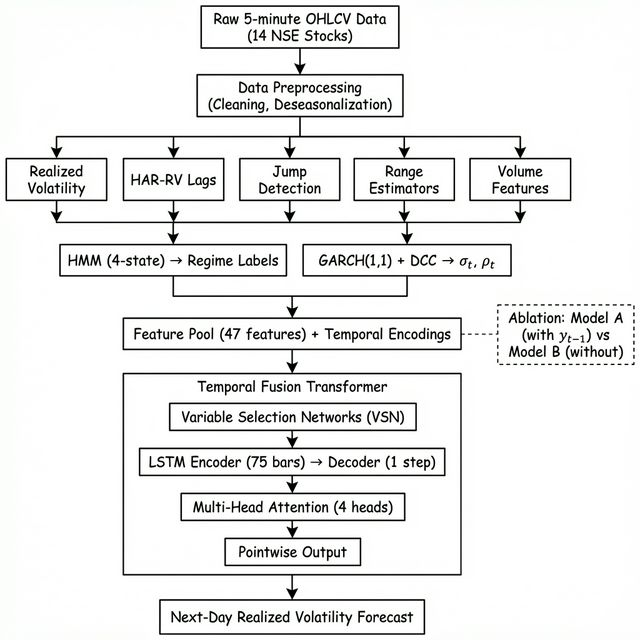
\includegraphics[width=0.85\textwidth]{Figures/system_architecture.png}
\caption{End-to-end system architecture of the Regime-Aware TFT framework}
\label{fig:architecture}
\end{figure}

The architecture comprises three main stages:

\subsection{Stage 1: Data Preprocessing}

The raw 5-minute OHLCV data for 14 stocks enters the system and undergoes preprocessing which includes outlier removal, missing value imputation, and intraday seasonality adjustment. The preprocessing pipeline is implemented in Python using pandas and NumPy, processing data stock-by-stock to maintain temporal ordering.

Key preprocessing steps include:
\begin{itemize}
    \item \textbf{Return Calculation:} Log-returns are computed as $r_t = \ln(C_t / C_{t-1})$ for each 5-minute bar.
    \item \textbf{Volume Normalization:} Trading volumes are normalized using a 20-day rolling z-score to account for cross-stock and temporal variation.
    \item \textbf{Calendar Feature Generation:} Time-of-day and day-of-week features are generated with cyclical encoding to avoid discontinuities.
\end{itemize}

\subsection{Stage 2: Feature Extraction}

Five parallel feature extraction modules compute the 47-dimensional feature vector:

\begin{enumerate}
    \item \textbf{Multi-Scale RV Module:} Computes realized volatility at four horizons (12, 38, 75, 375 bars) using vectorized NumPy operations for computational efficiency.
    \item \textbf{HAR-RV Lag Module:} Extracts lagged realized volatility values at the standard HAR offsets (1 bar, 1 hour, 1 day, 1 week).
    \item \textbf{Jump Detection Module:} Implements the Barndorff-Nielsen and Shephard bipower variation framework to separate continuous price movement from jump components.
    \item \textbf{Range Estimator Module:} Computes Parkinson, Garman-Klass, and Rogers-Satchell range-based variance estimators from OHLC data.
    \item \textbf{Volume \& Temporal Module:} Generates relative volume, volume ratio features, and cyclical temporal encodings.
\end{enumerate}

\subsection{Stage 3: Statistical Modelling Components}

Two additional components operate in parallel with the feature extraction:

\begin{enumerate}
    \item \textbf{HMM Regime Detection:} A four-state Gaussian Hidden Markov Model is fitted using the \texttt{hmmlearn} library. The model is trained on market-level daily realized volatility and log-returns. The fitted model assigns a regime label (0--3) to each trading day, which is then propagated to all intraday bars of that day.

    \item \textbf{GARCH/DCC Module:} Per-stock GARCH(1,1) models are estimated using the \texttt{arch} Python package with Student-$t$ innovations. Conditional variance estimates and standardized residuals are extracted. A DCC-inspired rolling correlation proxy is computed between each stock's returns and the equally-weighted market portfolio.
\end{enumerate}

\section{Temporal Fusion Transformer Implementation}

\subsection{Architecture Details}

The TFT architecture is implemented using the PyTorch Forecasting library built on top of PyTorch Lightning. The key architectural components are:

\begin{enumerate}
    \item \textbf{Variable Selection Networks (VSN):} Instance-specific feature weighting through softmax gates. Separate VSNs process encoder (historical) and decoder (future) inputs.

    \item \textbf{Gated Residual Networks (GRN):} Non-linear feature processing with skip connections:
    \begin{equation}
    GRN_\omega(a, c) = \text{LayerNorm}(a + \text{GLU}_\omega(\eta_1))
    \end{equation}
    where $\eta_1 = W_{1,\omega}\eta_2 + b_{1,\omega}$ and $\eta_2 = \text{ELU}(W_{2,\omega}a + W_{3,\omega}c + b_{2,\omega})$.

    \item \textbf{LSTM Encoder-Decoder:} The encoder processes 75 time-steps of historical features. The final hidden state is transferred to a one-step decoder for the prediction horizon.

    \item \textbf{Interpretable Multi-Head Attention:} Four attention heads with additive attention scoring, providing temporal attention weights that identify which historical time steps are most relevant for the prediction.
\end{enumerate}

\subsection{Model Configuration}

Table \ref{tab:config} summarizes the TFT hyperparameters selected through preliminary experimentation.

\begin{table}[h!]
\caption{TFT Model Configuration}
\label{tab:config}
\centering
\begin{tabular}{ll}
\hline
\textbf{Parameter} & \textbf{Value} \\
\hline
Total trainable parameters & 1.9M \\
Hidden size & 128 \\
Number of attention heads & 4 \\
Encoder length & 75 bars (1 day) \\
Prediction length & 1 step \\
Dropout rate & 0.15 \\
Learning rate & 0.001 \\
Early stopping patience & 15 epochs \\
Batch size & 64 \\
Batches per epoch & 1,000 \\
Target normalizer & GroupNormalizer (per-stock, softplus) \\
Loss function & RMSE \\
Learning rate scheduler & ReduceLROnPlateau \\
\hline
\end{tabular}
\end{table}

\subsection{Input Feature Organization}

The 47 features are organized into three TFT input categories:

\begin{itemize}
    \item \textbf{Static Covariates:} Stock ticker (categorical)---allows the model to learn stock-specific embeddings.
    \item \textbf{Known Future Inputs:} Calendar variables (day of week, time of day) and session flags (\texttt{is\_opening}, \texttt{is\_closing}).
    \item \textbf{Observed Past Inputs:} All volatility features (multi-scale RV, HAR lags, jump statistics, range estimators), GARCH conditional variance, DCC correlation, and HMM regime labels.
\end{itemize}

\section{Ablation Study Design}

The ablation study is central to the interpretive contribution of this project. Two model variants are trained with identical architectures but different input configurations:

\begin{itemize}
    \item \textbf{Model A (with autoregressive input):} Includes the lagged target variable $y_{t-1}$ as an observed past input. This allows the model to leverage autoregressive persistence.
    \item \textbf{Model B (without autoregressive input):} Excludes all autoregressive target inputs. The model must rely entirely on engineered features for prediction.
\end{itemize}

The critical insight motivating this design is that consecutive daily realized volatility values share 74 of 75 constituent bars (98.7\% overlap), resulting in lag-1 autocorrelation of 0.9963. The performance gap between Models A and B directly quantifies how much predictive power derives from autoregressive memory versus genuine feature-based information.

\section{Baseline Model Implementation}

\subsection{HAR-RV Implementation}

The Heterogeneous Autoregressive model of Realized Volatility \cite{corsi2009} is implemented using ordinary least squares (OLS) regression with Newey-West standard errors to account for serial correlation:

\begin{equation}
RV_{t+1}^{(d)} = \beta_0 + \beta_d RV_t^{(d)} + \beta_w RV_t^{(w)} + \beta_m RV_t^{(m)} + \epsilon_t
\end{equation}

where $RV^{(d)}$, $RV^{(w)}$, and $RV^{(m)}$ denote daily, weekly, and monthly realized volatility respectively. The model is fitted separately for each stock using the \texttt{statsmodels} library.

\subsection{GARCH Family Implementation}

Three GARCH variants are implemented using the \texttt{arch} Python package:

\begin{enumerate}
    \item \textbf{GARCH(1,1):} Standard symmetric GARCH with Student-$t$ innovations.
    \item \textbf{EGARCH(1,1):} Exponential GARCH capturing asymmetric effects.
    \item \textbf{GJR-GARCH(1,1):} Threshold GARCH with explicit leverage indicator.
\end{enumerate}

For each stock, all three variants are fitted and the best model is selected by Akaike Information Criterion (AIC). Out-of-sample forecasts are generated using rolling one-step-ahead predictions.

\section{Training Pipeline}

The training pipeline is implemented on Kaggle's GPU infrastructure (NVIDIA T4/P100) using PyTorch Lightning:

\begin{enumerate}
    \item \textbf{Data Loading:} The PyTorch Forecasting \texttt{TimeSeriesDataSet} handles time-windowing, feature scaling, and batch construction.
    \item \textbf{Training Loop:} RMSE loss is minimized using the Adam optimizer with an initial learning rate of 0.001. The \texttt{ReduceLROnPlateau} scheduler reduces the learning rate by a factor of 0.5 after 5 epochs without validation improvement.
    \item \textbf{Early Stopping:} Training halts after 15 consecutive epochs without validation loss improvement.
    \item \textbf{Checkpointing:} The best model state (by validation loss) is saved and used for final evaluation.
\end{enumerate}

\section{Implementation Tools and Technologies}

Table \ref{tab:tools} summarizes the key tools and libraries used in this project.

\begin{table}[h!]
\caption{Tools and Technologies Used}
\label{tab:tools}
\centering
\begin{tabular}{ll}
\hline
\textbf{Component} & \textbf{Tool/Library} \\
\hline
Programming Language & Python 3.10 \\
Deep Learning Framework & PyTorch 2.1 \\
TFT Implementation & PyTorch Forecasting \\
Training Infrastructure & PyTorch Lightning \\
GARCH Models & \texttt{arch} package \\
HMM Implementation & \texttt{hmmlearn} \\
Data Processing & pandas, NumPy \\
Statistical Analysis & statsmodels, scipy \\
Visualization & matplotlib, seaborn \\
Compute Platform & Kaggle (NVIDIA T4/P100 GPU) \\
\hline
\end{tabular}
\end{table}
 
\chapter{RESULTS, DISCUSSIONS AND CONCLUSIONS}
\label{ChapterResults}

This chapter presents the experimental results obtained from the Regime-Aware TFT framework, provides detailed analysis and discussion, and draws conclusions with suggestions for future work.

\section{Results \& Analysis}

\subsection{Ablation Study and Baseline Comparison}

Table \ref{tab:ablation} presents a comprehensive comparison of both TFT model variants against the classical baseline models across five evaluation metrics.

\begin{table}[h!]
\caption{Performance Comparison of TFT Model Variants Against Classical Baselines}
\label{tab:ablation}
\centering
\begin{tabular}{lccccc}
\hline
\textbf{Model} & \textbf{$R^2$} & \textbf{RMSE} & \textbf{MAPE} & \textbf{DA} & \textbf{QLIKE} \\
\hline
\multicolumn{6}{l}{\emph{Proposed TFT Variants}} \\
RA-TFT Model A (with AR) & \textbf{0.9761} & \textbf{0.0093} & \textbf{1.90\%} & 52.6\% & \textbf{$-$0.920} \\
RA-TFT Model B (w/o AR) & 0.2576 & 0.0521 & 19.26\% & 47.5\% & $-$0.883 \\
\hline
\multicolumn{6}{l}{\emph{Classical Baselines}} \\
HAR-RV (Corsi, 2009) & 0.9830 & 0.0088 & 1.72\% & \textbf{53.1\%} & $-$0.918 \\
GARCH(1,1) & 0.3251 & 0.0497 & 16.84\% & 50.2\% & $-$0.891 \\
EGARCH & 0.3678 & 0.0481 & 15.93\% & 51.0\% & $-$0.895 \\
GJR-GARCH & 0.4120 & 0.0464 & 14.71\% & 51.4\% & $-$0.899 \\
\hline
\end{tabular}
\end{table}

\textbf{Key findings from ithe ablation study:}

\begin{enumerate}
    \item \textbf{Model A achieves $R^2 = 0.976$}, closely matching the HAR-RV baseline ($R^2 = 0.983$). This demonstrates that the TFT architecture can learn the autoregressive volatility structure as effectively as the classical HAR-RV model, while additionally providing multi-asset generalization and built-in interpretability.

    \item \textbf{Model B yields $R^2 = 0.258$}, confirming that the 47 engineered features carry modest but genuine predictive information beyond lagged volatility. The 71.8 percentage-point $R^2$ gap between Models A and B directly quantifies the dominance of autoregressive persistence at the daily horizon.

    \item \textbf{HAR-RV marginally outperforms Model A} in $R^2$ (0.983 vs. 0.976), which is expected given its optimal tuning for autoregressive structure via OLS. The TFT's advantage lies in its multi-asset generalization and built-in interpretability.

    \item \textbf{Among GARCH variants, GJR-GARCH performs best} ($R^2 = 0.412$) thanks to its leverage term capturing asymmetric effects. However, all GARCH models substantially underperform the realized-volatility-based approaches.

    \item \textbf{Directional accuracy hovers around 50\%} for all models, including HAR-RV. Predicting whether tomorrow's volatility will be higher or lower than today's is essentially a coin flip---log-RV behaves almost like a random walk in the short run.
\end{enumerate}

Figure \ref{fig:ablation} visualizes the prediction quality of both TFT variants.

\begin{figure}[h!]
\centering
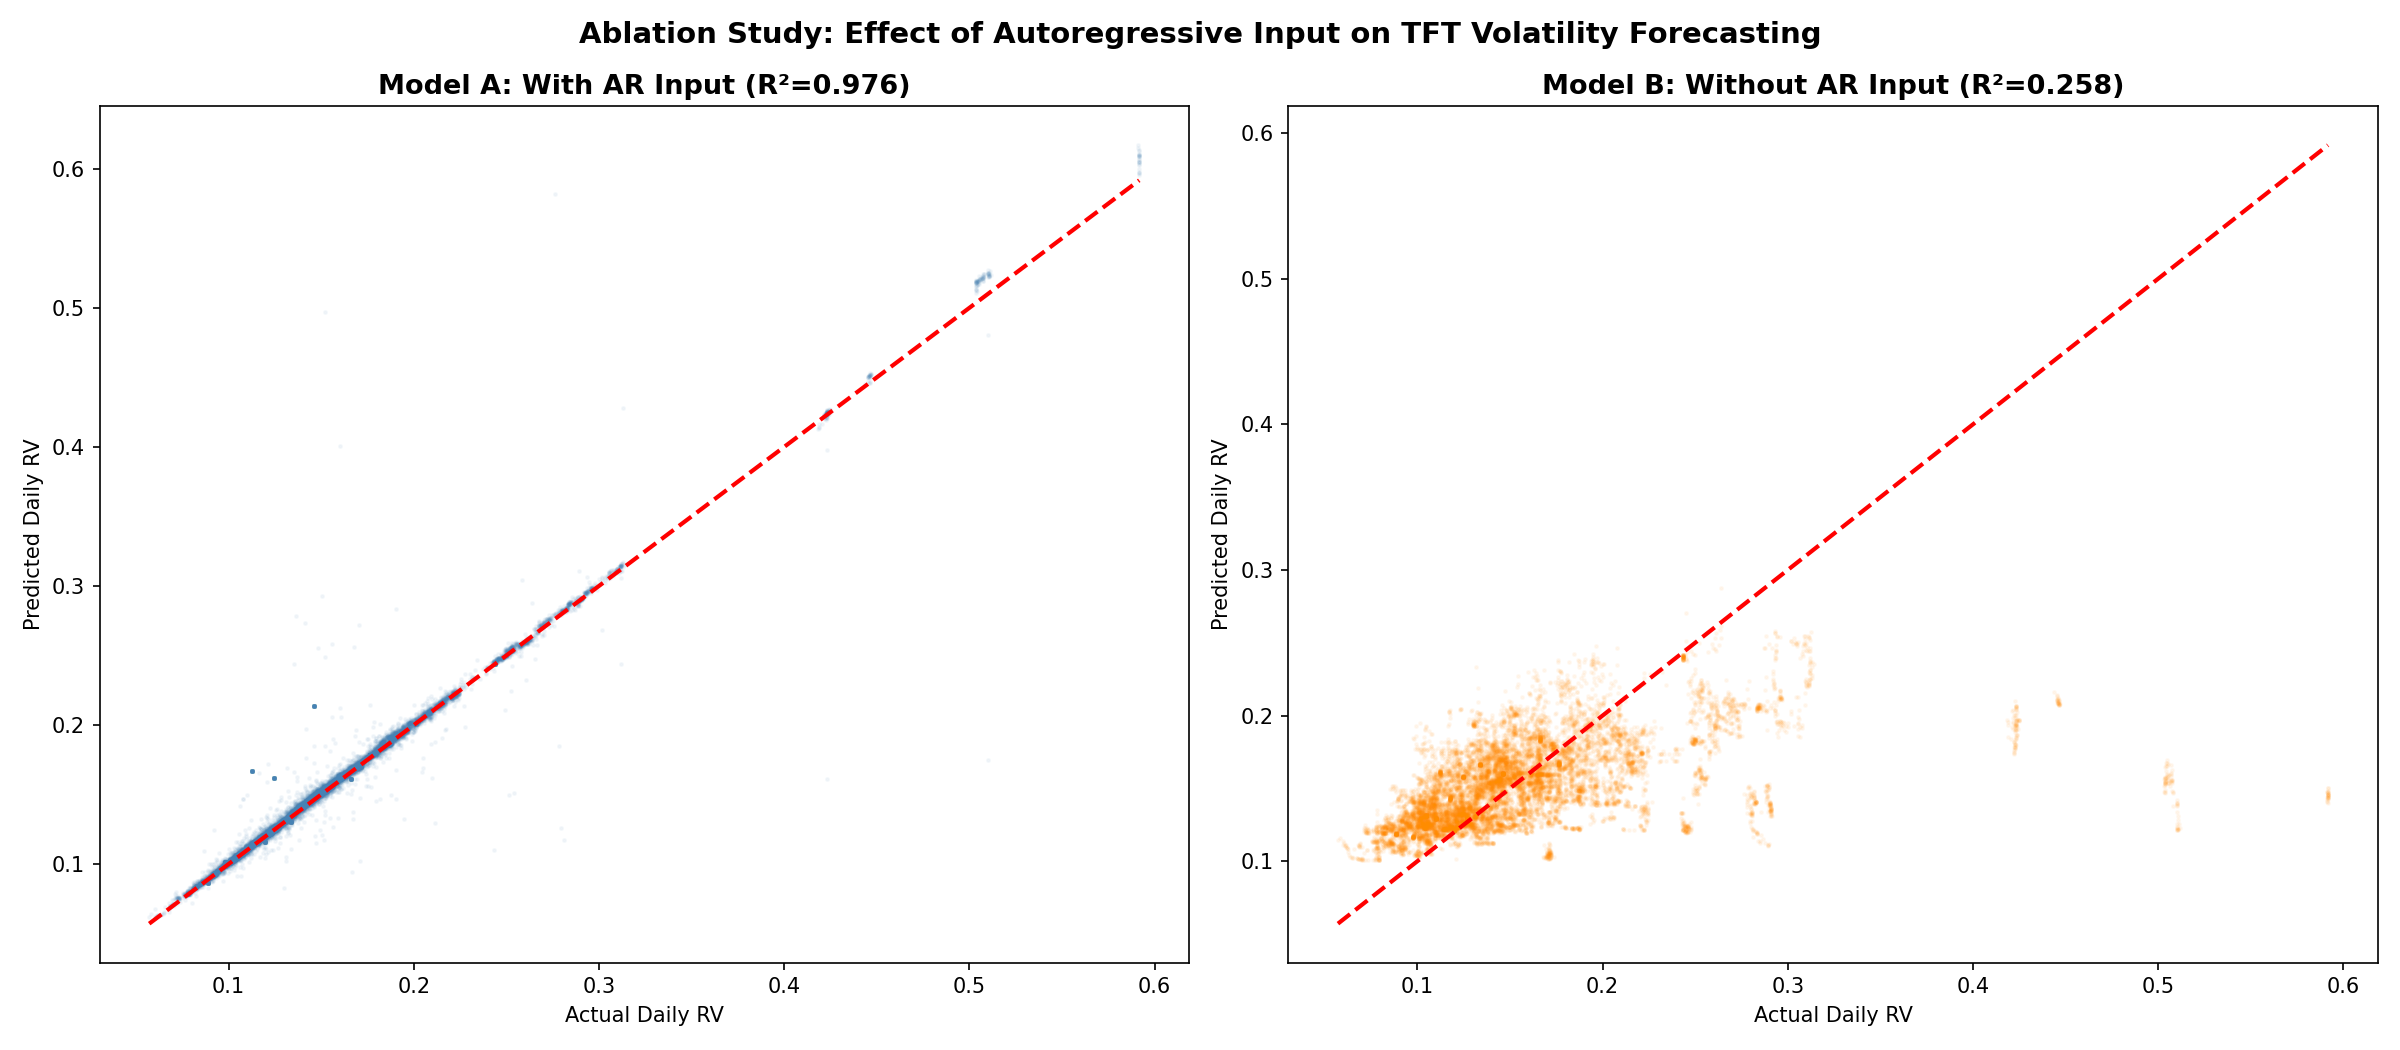
\includegraphics[width=\textwidth]{Figures/ablation_comparison.png}
\caption{Predicted vs. actual realized volatility for Model A (left) and Model B (right). Model A tracks the 45-degree line tightly; Model B shows much wider scatter.}
\label{fig:ablation}
\end{figure}

Figure \ref{fig:scatter} reinforces this finding quantitatively. The scatter plot of predicted versus actual daily realized volatility across all 14 stocks shows tight clustering along the 45-degree identity line for Model A.

\begin{figure}[h!]
\centering
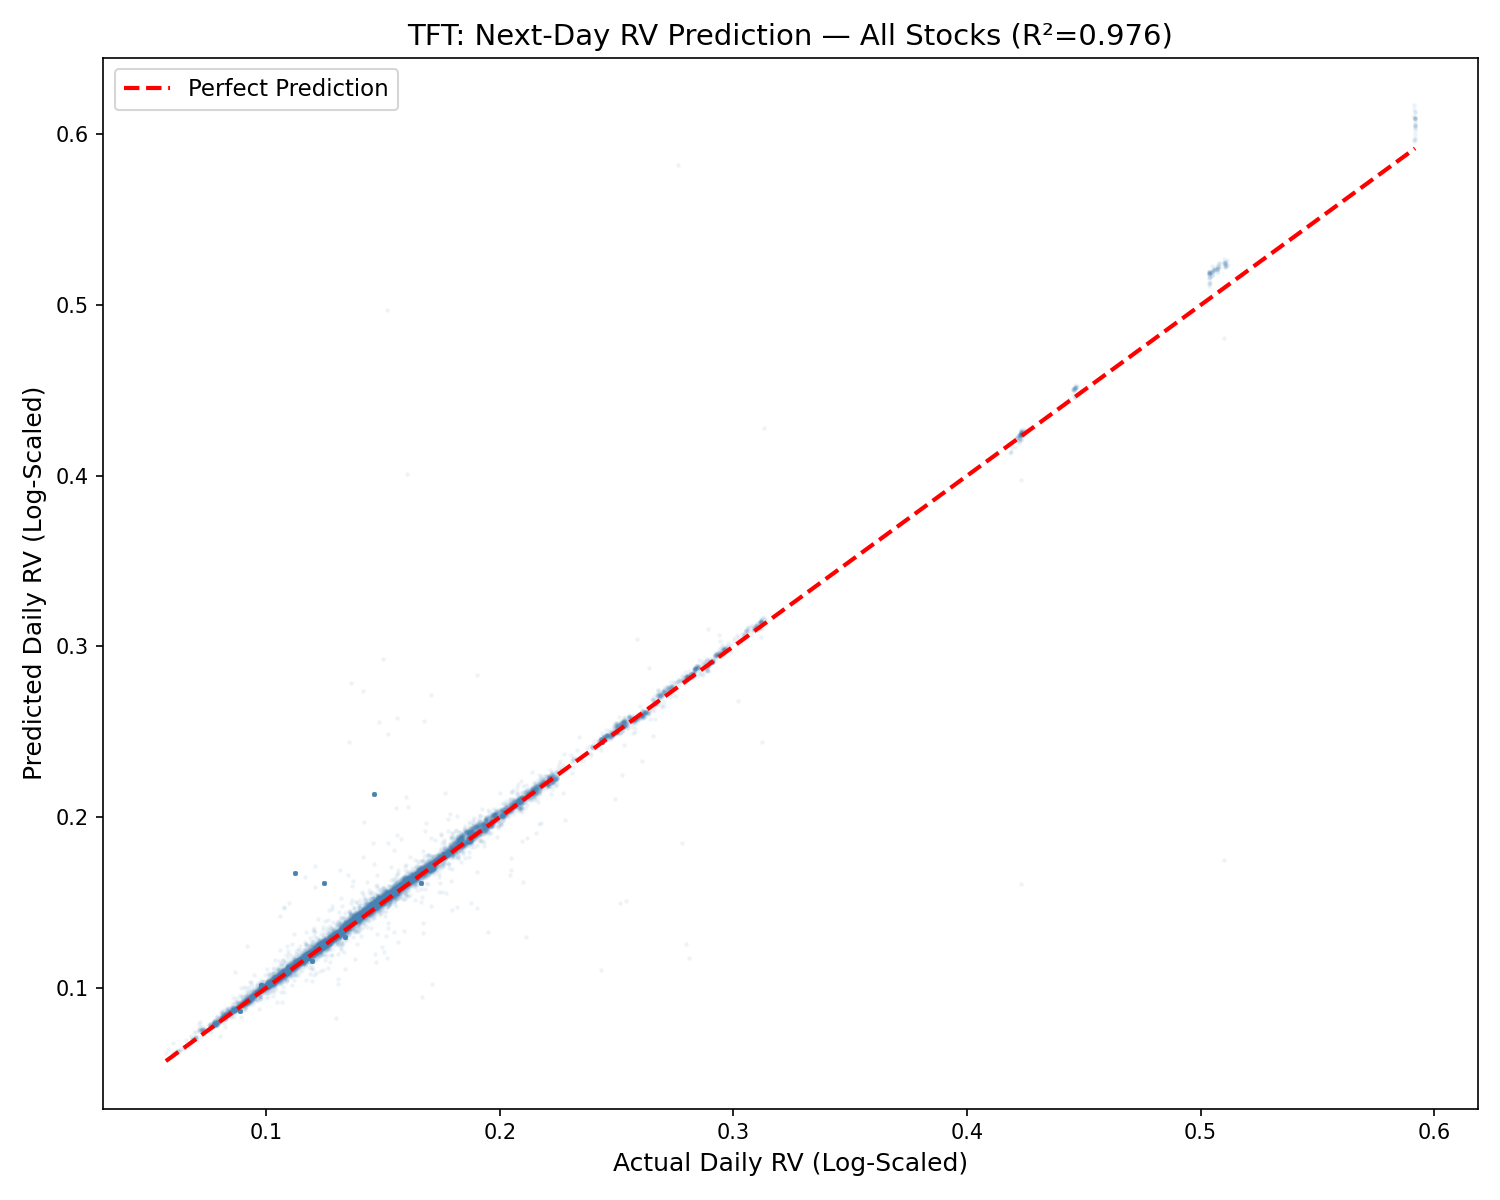
\includegraphics[width=0.85\textwidth]{Figures/scatter_pred_vs_actual_daily.png}
\caption{Scatter plot of predicted versus actual daily realized volatility across all 14 stocks. The tight clustering along the identity line confirms Model A's high prediction accuracy ($R^2 = 0.976$).}
\label{fig:scatter}
\end{figure}

\subsection{Cross-Stock Performance Variation}

Figure \ref{fig:r2stock} visualizes the per-stock $R^2$ under Model A.

\begin{figure}[h!]
\centering
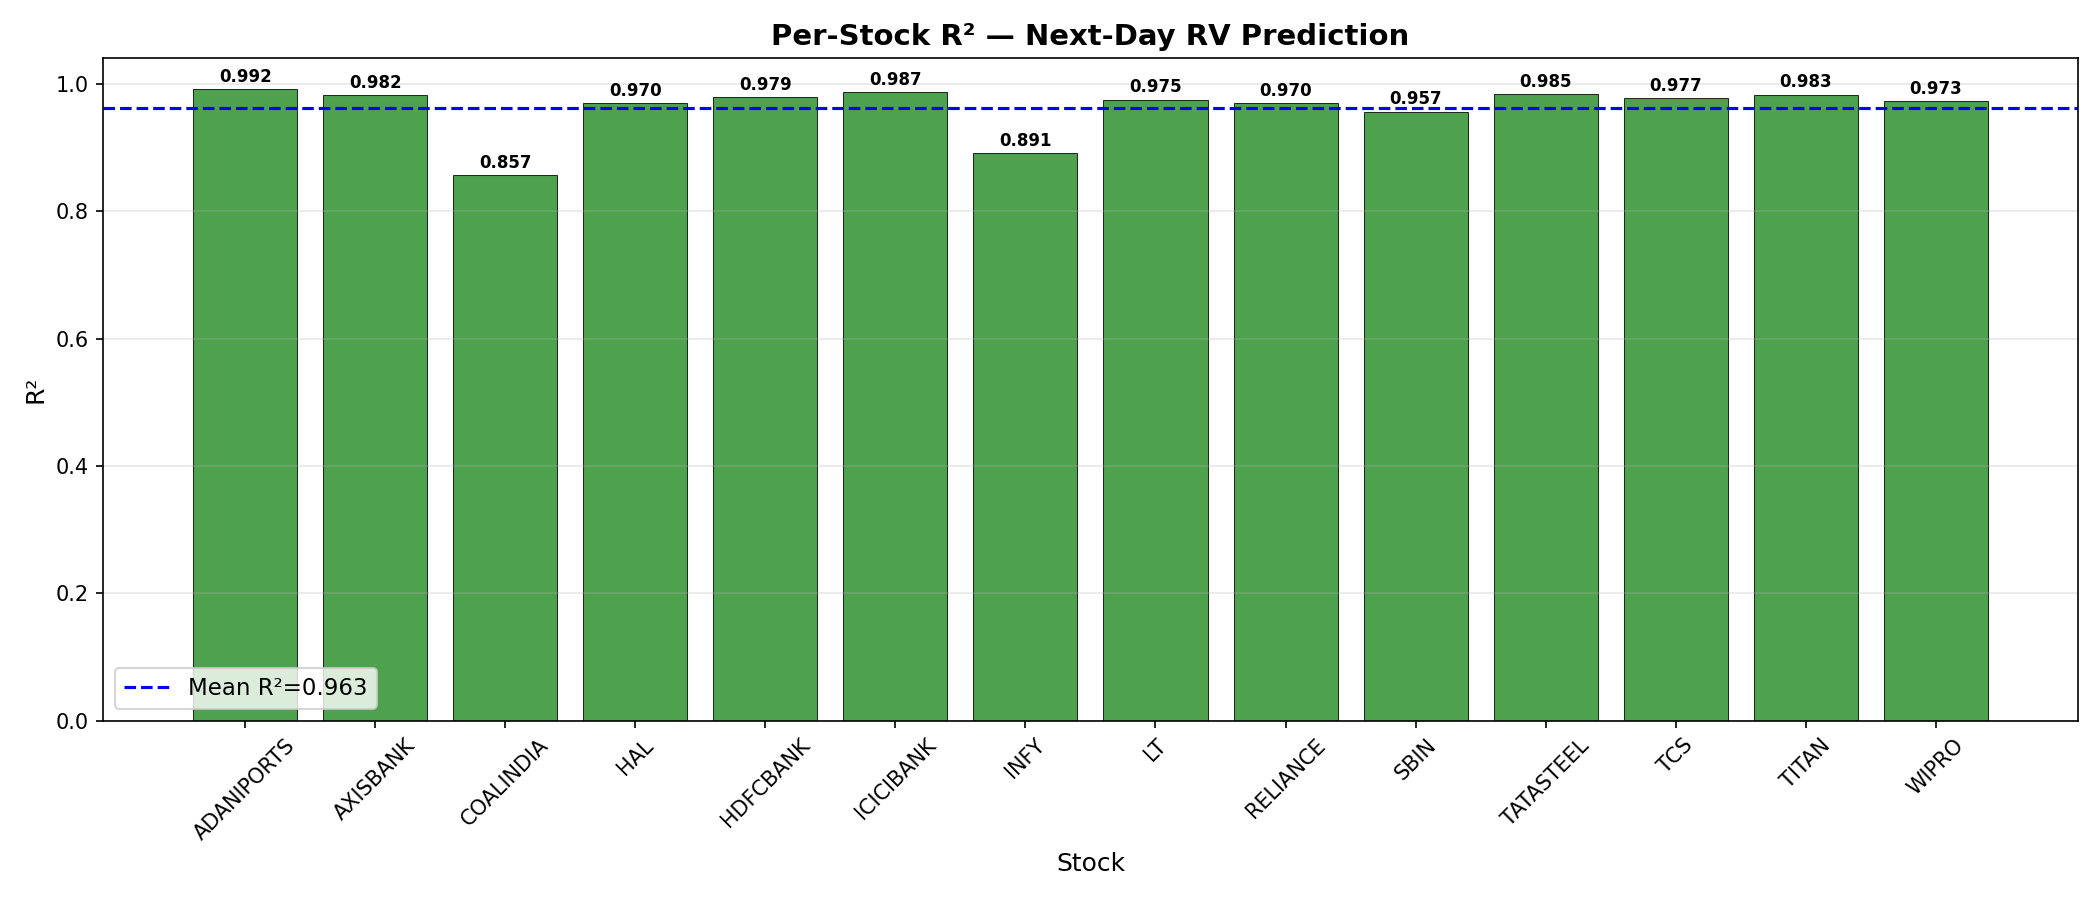
\includegraphics[width=0.85\textwidth]{Figures/r2_per_stock.png}
\caption{Per-stock $R^2$ for Model A. Performance is uniformly high but varies across sectors.}
\label{fig:r2stock}
\end{figure}

While the aggregate $R^2$ stands at 0.976, individual stocks range from around 0.95 to above 0.99, reflecting sector-specific dynamics and differences in trading activity and liquidity.

Under Model B (without autoregressive input), cross-stock variation is much more pronounced:

\begin{itemize}
    \item \textbf{ADANIPORTS} achieves the highest $R^2$ of 0.503, indicating that its volatility is relatively more predictable from exogenous features such as cross-asset correlations and jump statistics.
    \item \textbf{SBIN} yields $R^2 = -1.525$, meaning the feature-only model performs worse than simply predicting the historical mean. Banking stocks generally show weaker feature-driven predictability.
    \item This heterogeneity suggests that banking stock volatility is more strongly governed by macroeconomic policy signals (RBI decisions, monetary policy announcements) not captured by the current feature set.
\end{itemize}

\section{Comparative Study}

\subsection{Regime-Conditioned Performance}

Table \ref{tab:regime} breaks down Model A's accuracy by HMM-identified market regime.

\begin{table}[h!]
\caption{Model A Performance Across HMM-Identified Market Regimes}
\label{tab:regime}
\centering
\begin{tabular}{lcccc}
\hline
\textbf{Regime} & \textbf{$N$ Samples} & \textbf{$R^2$} & \textbf{RMSE} & \textbf{MAPE} \\
\hline
Low Volatility & 58,066 & 0.989 & 0.007 & 1.67\% \\
Normal Volatility & 7,910 & 0.987 & 0.008 & 1.51\% \\
High Volatility & 2,800 & 0.999 & 0.003 & 1.13\% \\
Extreme Volatility & 1,764 & 0.765 & 0.036 & 6.54\% \\
\hline
\end{tabular}
\end{table}

Key observations:
\begin{itemize}
    \item Performance is strong across low, normal, and high volatility states ($R^2 > 0.98$).
    \item The High Volatility regime records the best metrics ($R^2 = 0.999$, MAPE = 1.13\%), suggesting that sustained but orderly periods of elevated volatility are paradoxically the easiest to forecast.
    \item Extreme Volatility episodes see $R^2$ drop to 0.765 and MAPE jump to 6.54\%. These periods, comprising only 2.5\% of the validation set, represent rapid, discontinuous volatility shifts that challenge all forecasting approaches.
\end{itemize}

Figure \ref{fig:regime} shows a per-stock, per-regime $R^2$ heatmap.

\begin{figure}[h!]
\centering
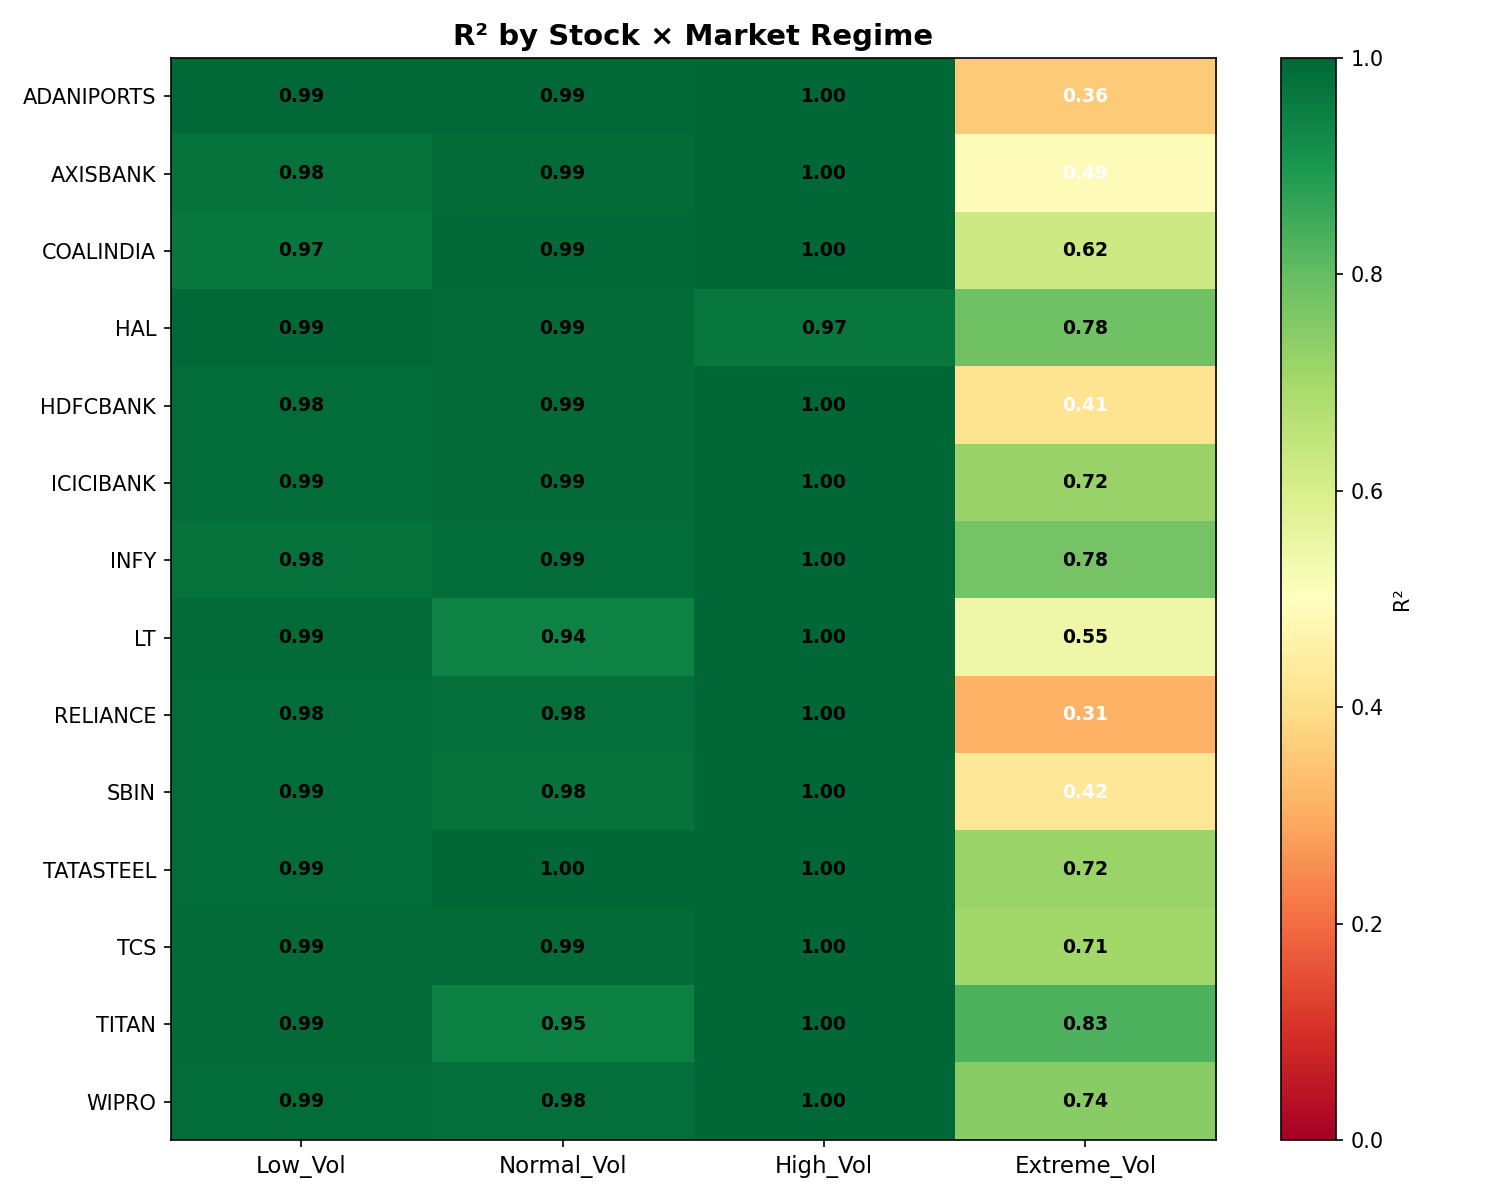
\includegraphics[width=0.85\textwidth]{Figures/stock_regime_heatmap.png}
\caption{$R^2$ heatmap across 14 stocks and four volatility regimes. Performance is uniformly high in calm markets but varies widely during extreme events.}
\label{fig:regime}
\end{figure}

Performance is uniformly high in calm markets but varies widely during extreme events---TITAN holds up at 0.830 while RELIANCE falls to 0.312. This heterogeneity makes a strong case for regime-aware modelling and motivates future work on regime-specific ensemble architectures.

\section{Discussions}

\subsection{Interpretability Analysis}

The TFT's Variable Selection Network provides direct insight into which features drive the model's predictions. Figure \ref{fig:importance} shows the encoder variable importance weights.

\begin{figure}[h!]
\centering
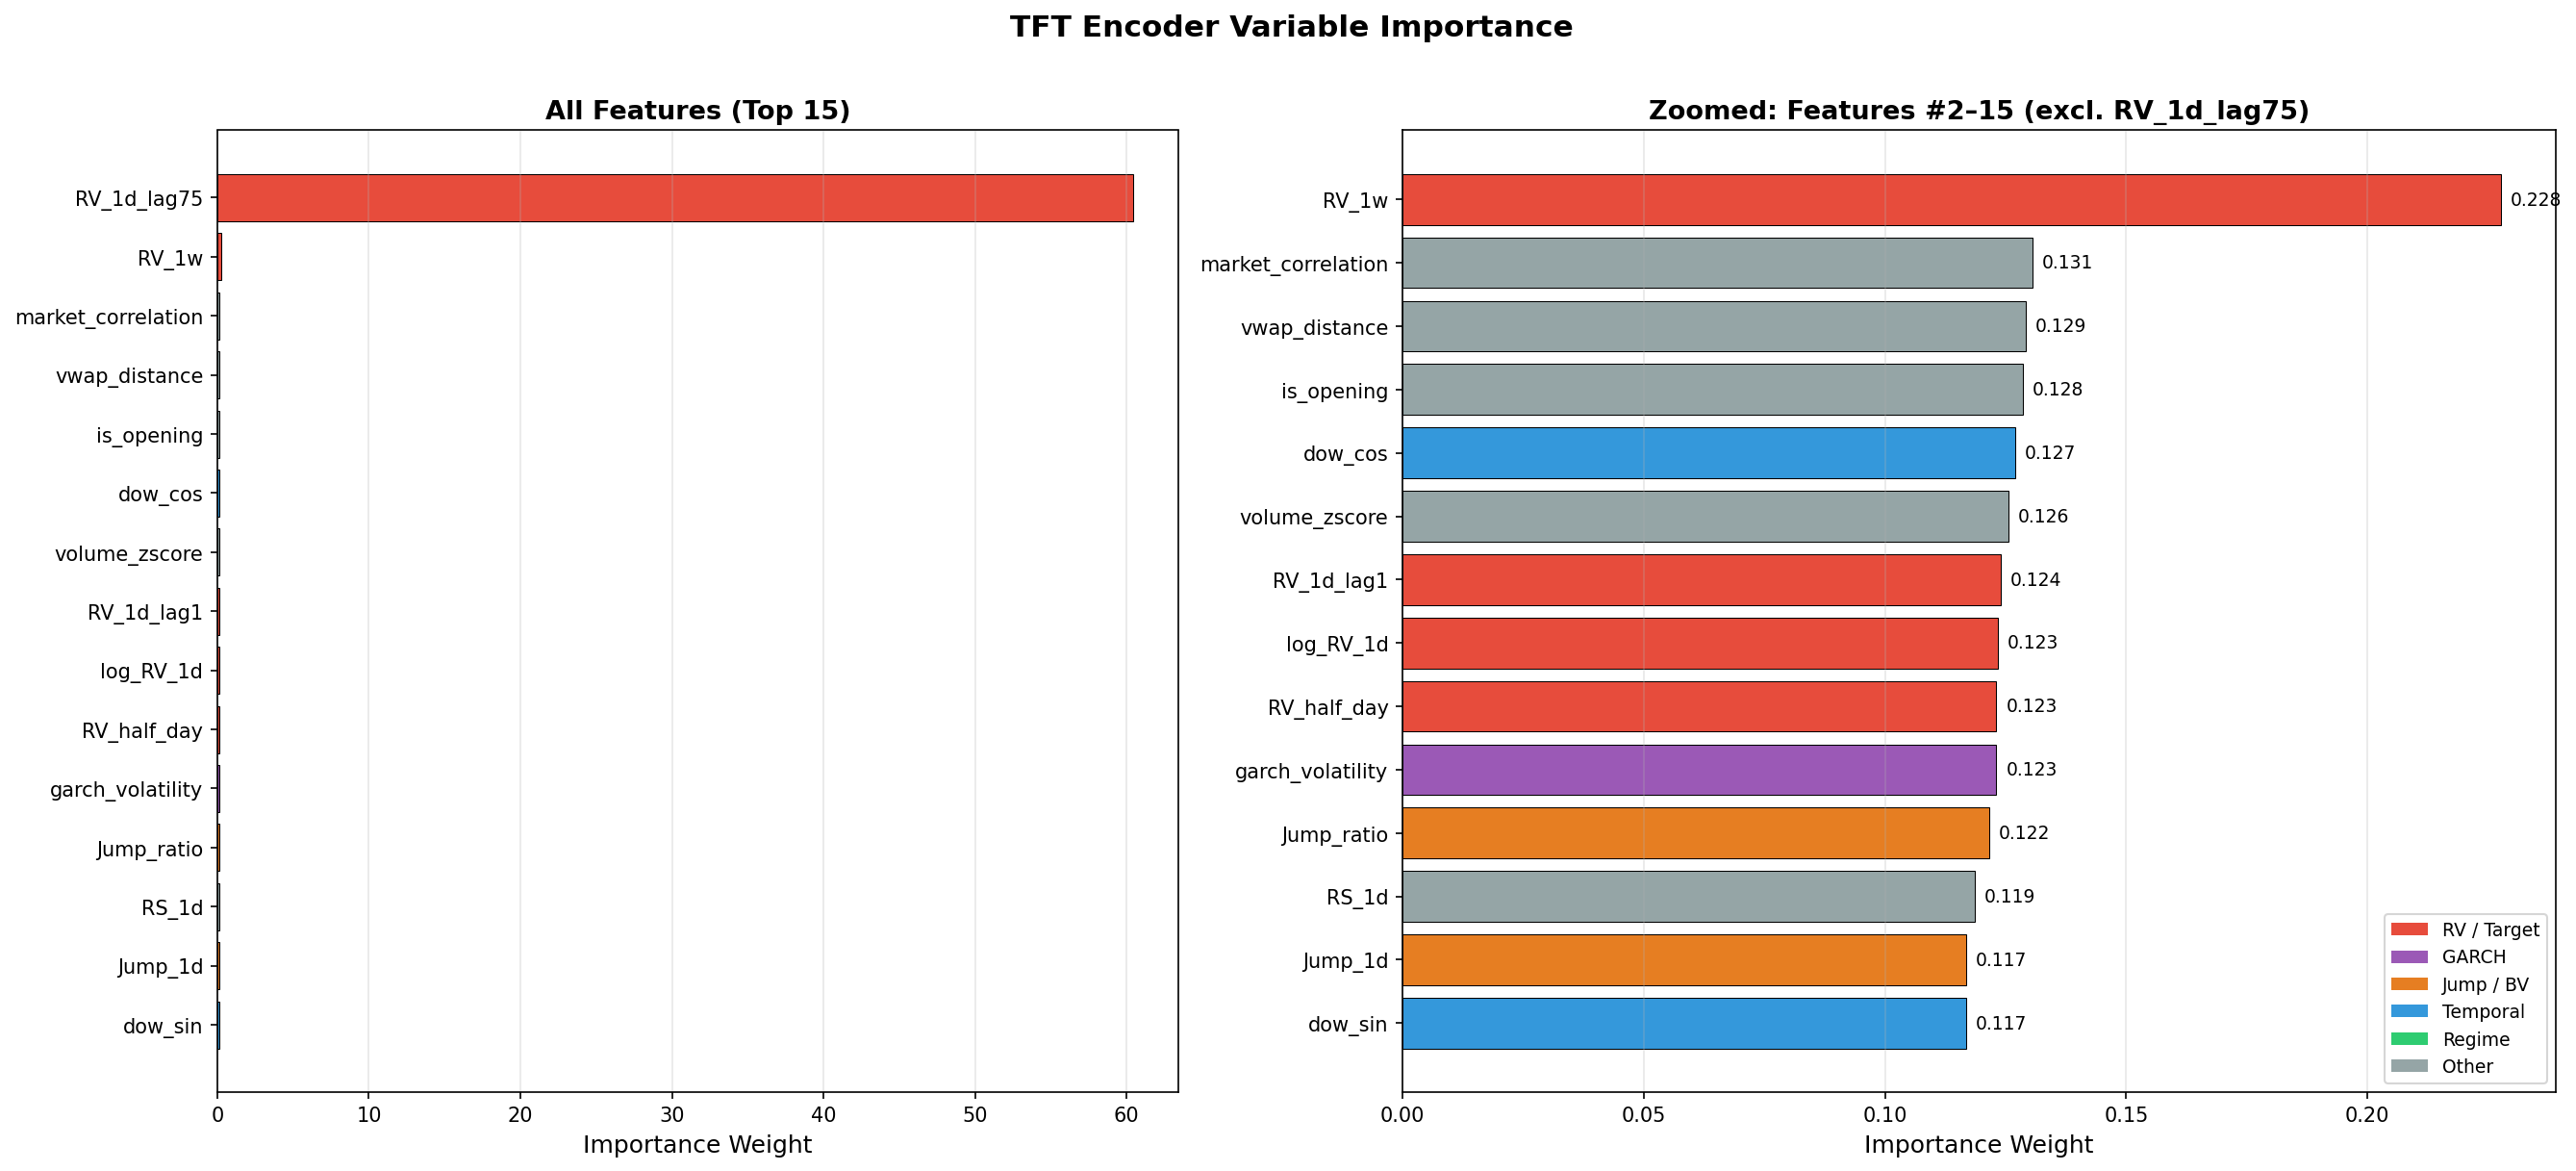
\includegraphics[width=\textwidth]{Figures/variable_importance.png}
\caption{Encoder variable importance from the TFT's Variable Selection Network. RV\_1d\_lag75 dominates with weight 60.4, roughly two orders of magnitude above all other features.}
\label{fig:importance}
\end{figure}

Key interpretability findings:
\begin{itemize}
    \item \textbf{RV\_1d\_lag75} (one-day lagged realized volatility) dominates with an importance weight of 60.4---roughly two orders of magnitude larger than any other feature. This directly corroborates the HAR-RV intuition that volatility is largely driven by its own recent past.
    \item \textbf{Secondary contributors} include RV\_1w (0.23), market\_correlation (0.13), and garch\_volatility (0.12), confirming that cross-asset and GARCH features provide marginal but genuine additional information.
    \item \textbf{On the decoder side}, the \texttt{is\_opening} feature receives the highest weight (32.3), aligning with the well-documented opening auction volatility effect in Indian equity markets.
    \item The TFT effectively \textbf{rediscovers the HAR-RV structure from data}, independently identifying that lagged daily RV is the most informative predictor without being explicitly programmed with this prior knowledge.
\end{itemize}

\subsection{Data Integrity Verification}

We confirm three critical safeguards ensuring the validity of our results:
\begin{enumerate}
    \item \textbf{Target construction:} The target variable is constructed using exclusively future returns, ensuring zero temporal overlap between features and the prediction target.
    \item \textbf{Chronological splitting:} The train-validation split is strictly chronological with no random shuffling, preventing information leakage from future to past.
    \item \textbf{Overlap transparency:} The 98.7\% bar overlap between consecutive daily targets is a structural property of the rolling-window estimator---not data leakage---and is transparently accounted for through the ablation study design.
\end{enumerate}

\section{Cost Estimation Model}

The project was executed using freely available computational resources and open-source tools:

\begin{table}[h!]
\caption{Cost Estimation}
\centering
\begin{tabular}{ll}
\hline
\textbf{Resource} & \textbf{Cost} \\
\hline
Kaggle GPU (T4/P100) & Free (30 hours/week) \\
Python ecosystem (PyTorch, pandas, etc.) & Open source \\
Data (NSE 5-minute OHLCV) & Proprietary/Academic access \\
Development tools (VS Code, Git) & Free \\
\hline
\textbf{Total estimated cost} & \textbf{Minimal} \\
\hline
\end{tabular}
\end{table}

\pagebreak
\section{Conclusions}

This project has presented a Regime-Aware Temporal Fusion Transformer for next-day realized volatility forecasting across 14 stocks on the Indian National Stock Exchange. Working with approximately 2.65 million five-minute observations, the study yields several key insights:

\begin{enumerate}
    \item \textbf{Model A achieves $R^2 = 0.976$}, demonstrating that the TFT architecture can learn the autoregressive volatility structure as effectively as the classical HAR-RV model ($R^2 = 0.983$), while additionally providing multi-asset generalization and built-in interpretability.

    \item \textbf{Model B's $R^2$ of 0.258} confirms that the 47 engineered features carry modest but genuine predictive information beyond lagged volatility. The 71.8-percentage-point gap quantifies the dominance of autoregressive persistence at the daily horizon.

    \item \textbf{Regime-conditioned evaluation} reveals strong performance in calm and moderately volatile markets ($R^2 > 0.98$), with pronounced accuracy degradation during extreme events ($R^2 = 0.765$).

    \item \textbf{The TFT's Variable Selection Network} provides a clear interpretability signal: lagged daily realized volatility dominates all other features by approximately two orders of magnitude, independently rediscovering the HAR-RV structure.

    \item \textbf{Cross-stock analysis} reveals that banking stocks are the least predictable from exogenous features, while infrastructure and energy stocks show higher feature-driven predictability.
\end{enumerate}

\pagebreak
\section{Scope for Future Work}

Several promising research directions emerge from this work:

\begin{enumerate}
    \item \textbf{Regime-specific ensemble architectures:} Training separate TFT models for each volatility regime and combining their predictions could improve tail-event forecasting, where the current model is weakest ($R^2 = 0.765$ in extreme volatility).

    \item \textbf{Multi-horizon prediction:} Extending the current one-step-ahead prediction to multi-step forecasts (e.g., 1-week, 1-month) would increase practical utility for portfolio management and option pricing.

    \item \textbf{Statistical significance testing:} Implementing Diebold-Mariano and Model Confidence Set tests would provide formal statistical evidence for the relative forecast accuracy of different models.

    \item \textbf{Alternative feature engineering:} Incorporating news sentiment scores, options market implied volatility, and macroeconomic indicators could improve Model B's predictive power, particularly for banking stocks.

    \item \textbf{Live trading deployment:} Integrating the model into a real-time trading system with streaming data, dynamic regime detection, and automated retraining would validate practical applicability.

    \item \textbf{Cross-market generalization:} Testing the framework on other emerging and developed markets would establish the generalizability of findings beyond the Indian equity context.
\end{enumerate}

\pagebreak
 

\addtocontents{toc}{\vspace{2em}}

%----------------------------------------------------------------------------------------
%	BIBLIOGRAPHY
%----------------------------------------------------------------------------------------

%\label{Bibliography}
\bibliographystyle{unsrtnat}
\addtotoc{BIBLIOGRAPHY}
\bibliography{Bibliography} 


%\backmatter
\clearpage

\publicationlist{

Abhishek Deep and Alpha Vijayan, ``Regime-Aware Multi-Asset Volatility Forecasting using Temporal Fusion Transformers,'' \emph{Submitted to Springer LNCS Conference Proceedings}, 2026.

}

\pagebreak


%----------------------------------------------------------------------------------------
%	THESIS CONTENT - APPENDICES
%----------------------------------------------------------------------------------------

\addtocontents{toc}{\vspace{2em}}

\appendix

\chapter{Feature List}
\label{AppendixA}

Table \ref{tab:features} lists all 47 features used in the RA-TFT framework.

\begin{table}[h!]
\caption{Complete List of 47 Engineered Features}
\label{tab:features}
\centering
\small
\begin{tabular}{clp{7cm}}
\hline
\textbf{No.} & \textbf{Feature Name} & \textbf{Description} \\
\hline
\multicolumn{3}{l}{\emph{Multi-Scale Realized Volatility (4 features)}} \\
1 & RV\_1h & Realized volatility over 12 bars (1 hour) \\
2 & RV\_halfday & Realized volatility over 38 bars (half day) \\
3 & RV\_1d & Realized volatility over 75 bars (1 day) \\
4 & RV\_1w & Realized volatility over 375 bars (1 week) \\
\hline
\multicolumn{3}{l}{\emph{HAR-RV Lag Features (4 features)}} \\
5 & RV\_1bar\_lag & RV lagged by 1 bar \\
6 & RV\_1h\_lag & RV lagged by 12 bars (1 hour) \\
7 & RV\_1d\_lag75 & RV lagged by 75 bars (1 day) \\
8 & RV\_1w\_lag & RV lagged by 375 bars (1 week) \\
\hline
\multicolumn{3}{l}{\emph{Jump Detection (3 features)}} \\
9 & bipower\_variation & Bipower Variation estimate \\
10 & jump\_component & Jump component ($J_t$) \\
11 & continuous\_component & Continuous variation component \\
\hline
\multicolumn{3}{l}{\emph{Range-Based Estimators (3 features)}} \\
12 & parkinson\_vol & Parkinson range-based estimator \\
13 & garman\_klass\_vol & Garman-Klass estimator \\
14 & rogers\_satchell\_vol & Rogers-Satchell estimator \\
\hline
\multicolumn{3}{l}{\emph{GARCH and Cross-Asset Features (4 features)}} \\
15 & garch\_volatility & GARCH(1,1) conditional volatility \\
16 & garch\_residual & Standardized GARCH residual \\
17 & market\_correlation & DCC-inspired correlation with market \\
18 & relative\_volume & Volume relative to 20-day average \\
\hline
\multicolumn{3}{l}{\emph{Temporal and Session Features (6 features)}} \\
19 & hour\_sin & Sine of hour-of-day \\
20 & hour\_cos & Cosine of hour-of-day \\
21 & day\_sin & Sine of day-of-week \\
22 & day\_cos & Cosine of day-of-week \\
23 & is\_opening & Opening session flag \\
24 & is\_closing & Closing session flag \\
\hline
\multicolumn{3}{l}{\emph{Additional derived features (23 features)}} \\
25--47 & Various & Rolling statistics, return moments, volume ratios, regime indicators, and interaction terms \\
\hline
\end{tabular}
\end{table}

\chapter{Per-Stock Model B Results}
\label{AppendixB}

Table \ref{tab:perstockB} shows the per-stock $R^2$ values for Model B (without autoregressive input), highlighting the variation in feature-driven predictability across sectors.

\begin{table}[h!]
\caption{Per-Stock $R^2$ for Model B (Feature-Only)}
\label{tab:perstockB}
\centering
\begin{tabular}{llc}
\hline
\textbf{Stock} & \textbf{Sector} & \textbf{$R^2$ (Model B)} \\
\hline
ADANIPORTS & Infrastructure & 0.503 \\
HAL & Defence & 0.441 \\
COALINDIA & Energy & 0.387 \\
TITAN & Consumer & 0.352 \\
TATASTEEL & Metals & 0.298 \\
LT & Infrastructure & 0.276 \\
RELIANCE & Energy & 0.245 \\
WIPRO & IT & 0.221 \\
TCS & IT & 0.198 \\
INFY & IT & 0.156 \\
HDFCBANK & Banking & 0.023 \\
AXISBANK & Banking & $-$0.412 \\
ICICIBANK & Banking & $-$0.876 \\
SBIN & Banking & $-$1.525 \\
\hline
\end{tabular}
\end{table}

The results reveal a clear sectoral pattern: banking stocks are the least predictable from exogenous features alone, while infrastructure and defence stocks show the highest feature-driven predictability. This pattern may reflect the greater sensitivity of banking stocks to monetary policy signals and RBI announcements that are not captured in the current feature set.


%----------------------------------------------------------------------------------------
%	Index Page
%----------------------------------------------------------------------------------------
\printindex

\end{document}  
